\documentclass{article}
\usepackage[UTF8]{ctex}
\usepackage{geometry}
\usepackage{makecell}
\usepackage{amsmath}
\usepackage{graphicx}
\usepackage{bigstrut}
\usepackage{subfigure}
\usepackage{float}
\usepackage{booktabs}
\usepackage{hyperref}
\usepackage{xcolor}
\definecolor{linkcolour}{rgb}{0,0.2,0.6}
\hypersetup{colorlinks,breaklinks,urlcolor=linkcolour, linkcolor=linkcolour}

\geometry{a4paper,scale=0.75}

\title{\heiti 实验三十六\ 光源的时间相干性}
\author{\kaishu 田睿轩\ 物理学院\ 1900011602}
\date{2021年6月8日}
\newcommand{\degree}{^\circ}
\newcommand{\degreesCelsius}{^\circ C}

\begin{document}
    \maketitle
    \section{数据处理}
    \subsection{白光相干长度}
    调出白光等厚干涉,从白光条纹的对称中心置于视场中心,此时即为等光程处,M1镜位置读数为$d_0=48.645mm$。
    向两侧数白光条纹,除了对称中心的0级条纹,只能看到1级白色条纹,因此有$k_1=1$,于是可计算白光相干长度$\Delta L_{1 \max }$
    $$\Delta L_{1 \max } \approx k_{1} \lambda_{1}=1\times 550nm=0.55\mu m$$

    根据白光的相干长度计算其相干时间
    $$t_=\frac{\Delta L_{1\max }}{c}=\frac{0.55\times 10^{-6}}{3\times 10^8}=1.8\times 10^{-15}s$$

    \subsection{橙色光相干长度}
    在光源前加上橙色玻璃滤光,测量橙色光的相干长度。用微调旋钮改变光程差,数移过视场中心的条纹数直到看不到条纹,
    总共数到$k_2\approx 18$条,由此得橙光相干长度$\Delta L_{2 \max }$
    $$\Delta L_{2 \max } \approx k_{2} \lambda_{2}=18\times 625nm=11.25\mu m$$

    计算得橙色光的相干时间为
    $$t_2=\frac{\Delta L_{2\max }}{c}=\frac{11.25\times 10^{-6}}{3\times 10^8}=3.8\times 10^{-14}s$$

    \subsection{黄色光的相干长度}
    用黄色滤光片对白光滤光。同样用微调旋钮改变光程,数移过视场中心的条纹数直到看不到条纹,共有$k_3\approx 57$条,因此黄光的相干长度$\Delta L_{3 \max }$为
    $$\Delta L_{3 \max } \approx k_{3} \lambda_{3}=57\times 578nm=32.95\mu m$$

    黄光相干时间为
    $$t_3=\frac{\Delta L_{3\max }}{c}=\frac{32.95\times 10^{-6}}{3\times 10^8}=1.1\times 10^{-13}s$$

    \subsection{汞灯黄光的相干长度}
    用低压汞灯照明并加上黄色滤光片,由于汞黄光为双线光,相干长度较长,所以不能用上述等厚干涉数条纹的方式测量,要用等倾干涉来测量
    从等光程处开始改变光程,可以看到条纹可见度发生周期性变化,即“拍”的现象。同时可见度越来越小,直到达到某一位置时条纹不可见,此位置的刻度为$d_{max}=95.001mm$,
    由此可得汞黄光的相干长度为
    $$\Delta L_{4 \max }=2 \left( d_{\max }-d_{0} \right)=2\times (95.001-48.645)=9.27cm$$

    汞黄光的相干时间为
    $$t_4=\frac{\Delta L_{4\max }}{c}=\frac{9.27\times 10^{-2}}{3\times 10^8}=3.1\times 10^{-10}s$$

    \subsubsection{汞黄光的波长差$\Delta \lambda$}
    \subsubsection{方法一}
    由于汞黄光为双线光,干涉条纹的总强度是这两套光的非相干叠加,因此条纹可见度会随光程做周期性变化。
    从等光程处开始改变光程,条纹可见度从清晰到消失再到清晰,呈周期性变化,出现“拍”的现象。通过测量拍的两个相邻节点之间的距离$\Delta d$,
    可以计算出波长差$\Delta \lambda$。实验中,从等光程处开始连续记录7个条纹可见度为0的的位置的M1镜的读数,然后用最小二乘法拟合得到拍的相邻两个节点之间的距离。
    实验数据如表1所示。最小二乘法拟合结果如图1所示。

    \begin{table}[htbp]
        \centering
        \caption{相邻拍节点的位置}
        \vspace{1ex}
        \begin{tabular}{cccccccc}
          \toprule
          拍的节点  & 1     & 2     & 3     & 4     & 5     & 6     & 7 \\
          $d_i/mm$ & 48.687 & 48.76 & 48.838 & 48.91 & 48.985 & 49.07 & 49.158 \\
          \bottomrule
        \end{tabular}%
    \end{table}%

    \begin{figure*}[htbp]
        \centering
        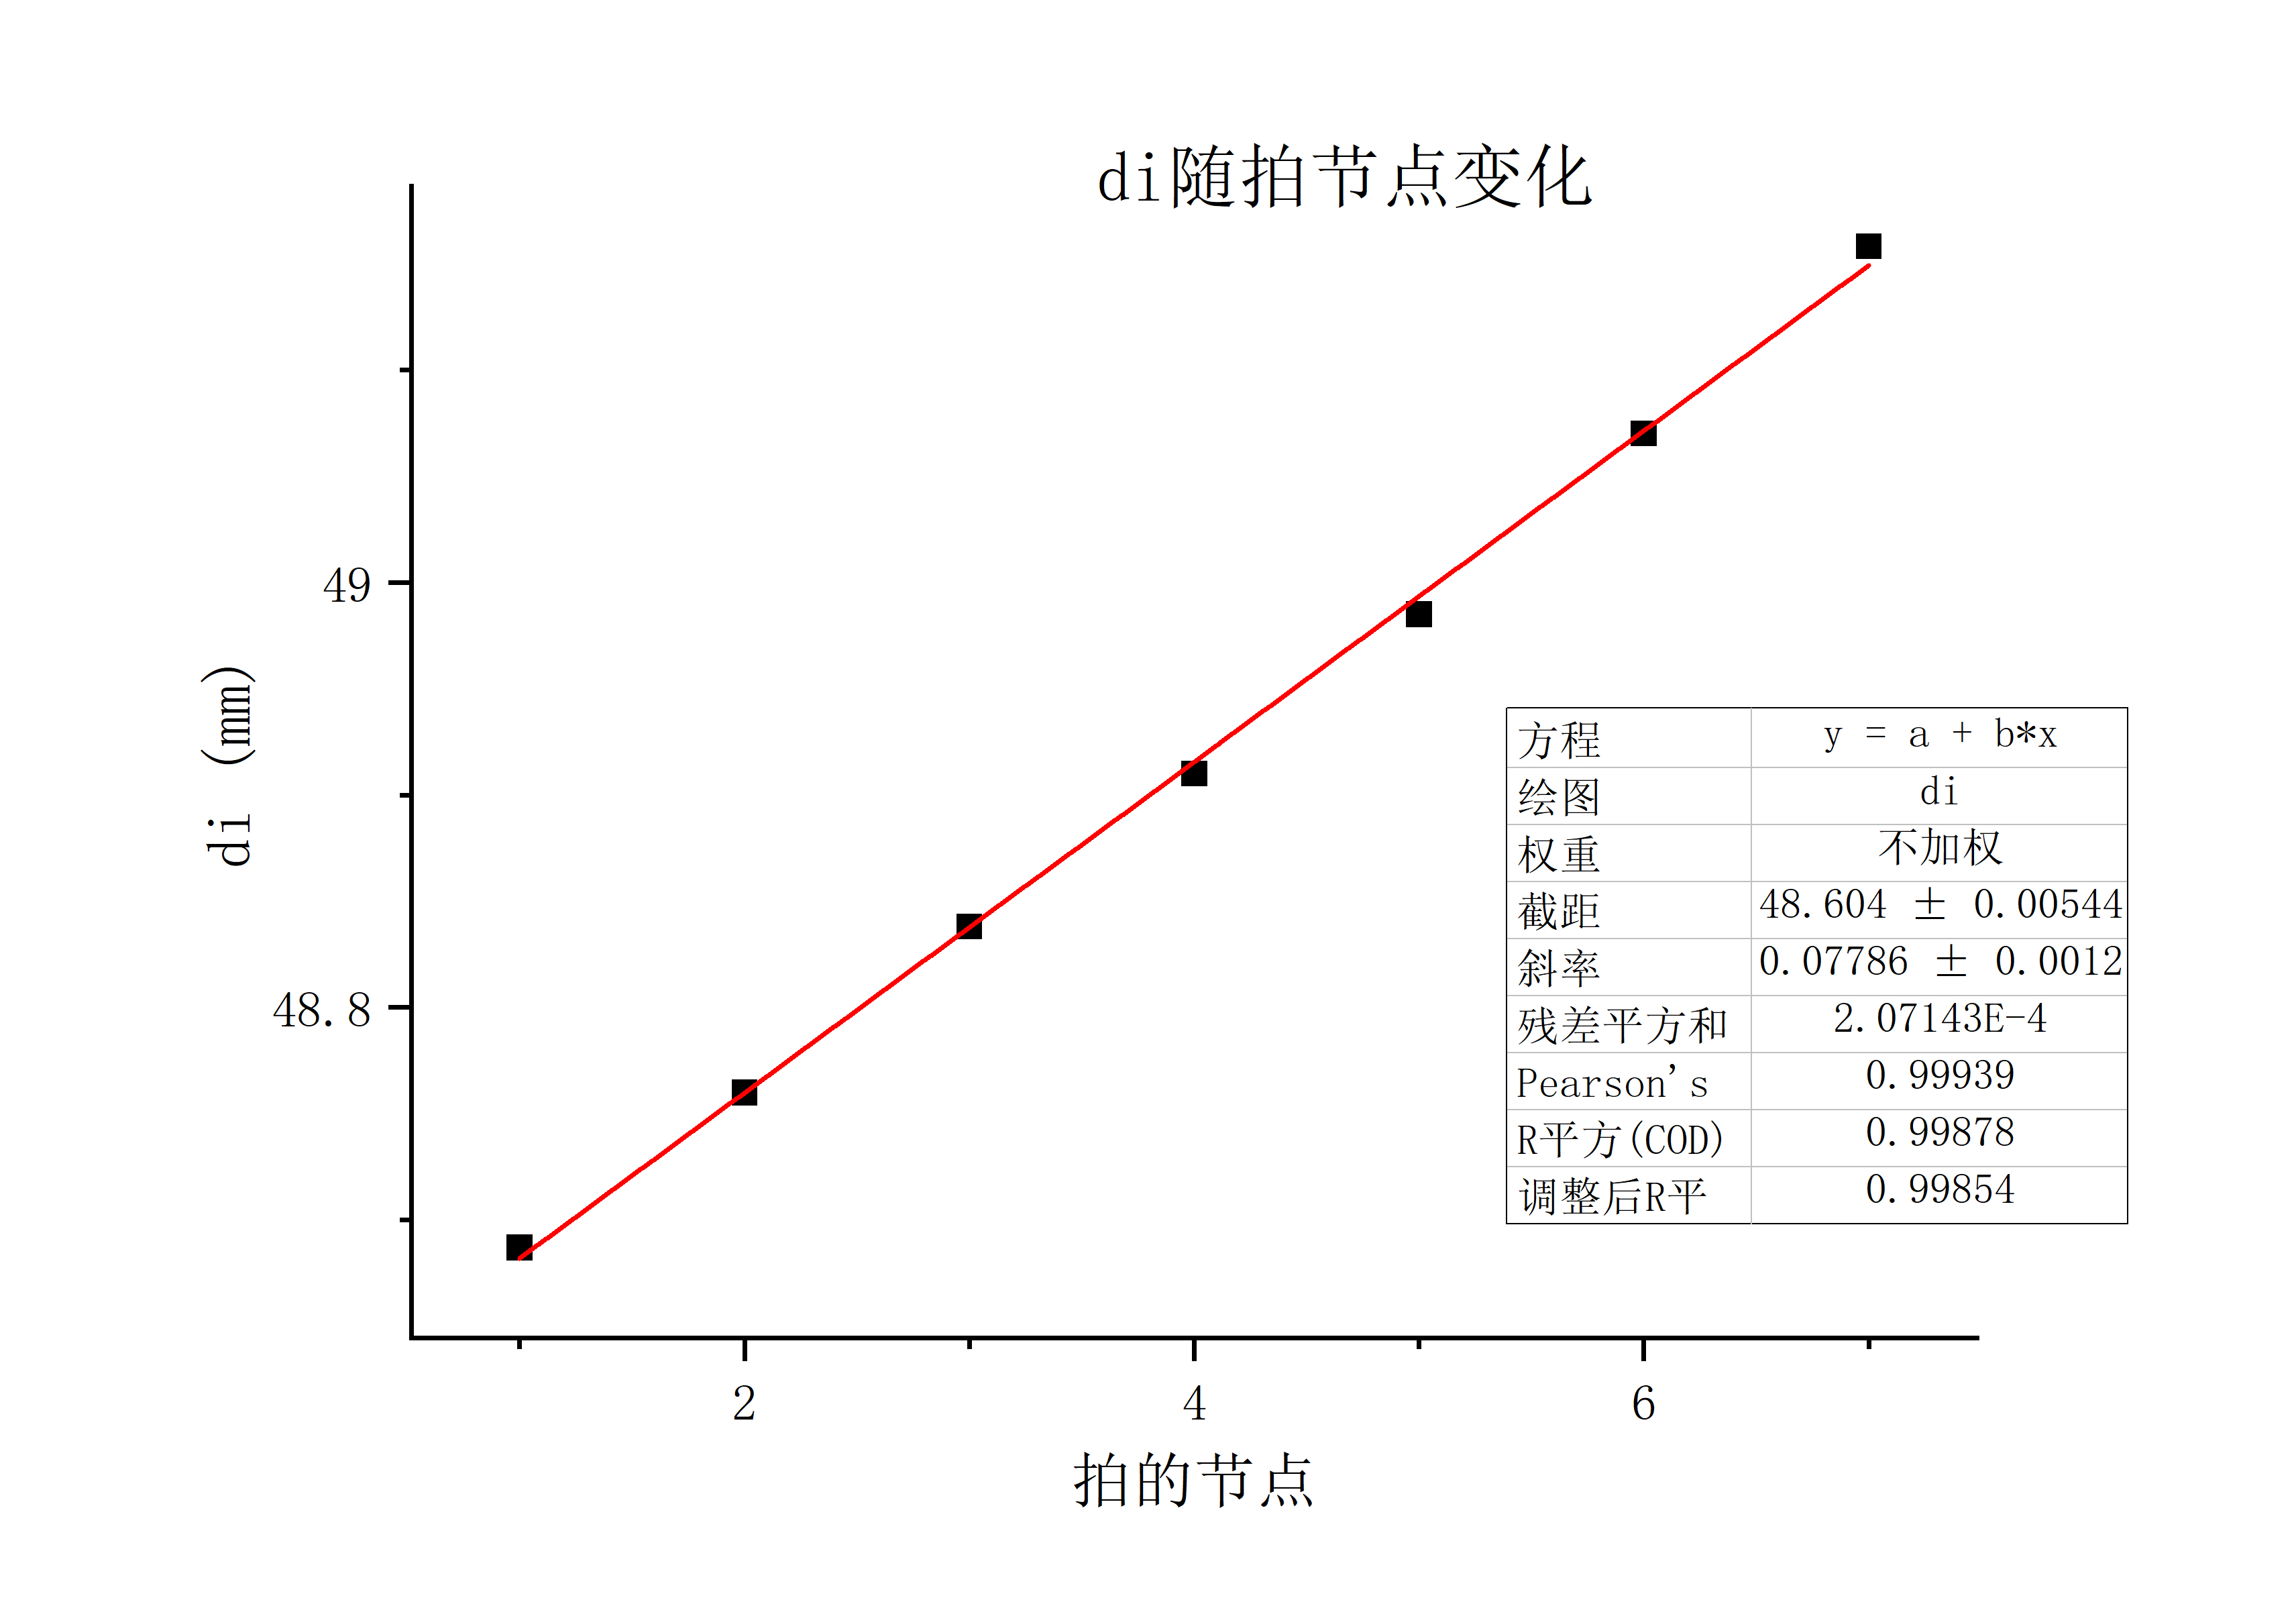
\includegraphics[width=0.62\textwidth]{di随节点变化.jpg}
        \caption{$d_i$随拍的节点变化}
    \end{figure*}

    最小二乘法拟合出的直线斜率即为相邻两个拍节点之间的距离$\Delta d=0.078mm$,通过滤光片获得的黄光波长取$\lambda=578nm$,可得汞黄光的波长差
    $$\Delta \lambda \equiv \lambda_{2}-\lambda_{1} \approx \frac{\lambda}{\Delta k} \approx \frac{\lambda^{2}}{2 \Delta d}=\frac{578^2}{2\times 0.078\times 10^6}=2.14nm$$

    \subsubsection{方法二}
    利用实验室提供的汞黄双线的干涉图,可以直接数出两相邻的可见度为零的区间内,干涉条纹的数目$\Delta k$。
    实验中提供了两个干涉图,其中一个干涉图中数出的条纹数目$\Delta k_1=271$,另一个为$\Delta k_2=273$。
    因此
    $$\overline{\Delta k}=\frac{\Delta k_1+\Delta k_2}{2}=272$$
    $$\Delta \lambda \equiv \lambda_{2}-\lambda_{1} \approx \frac{\lambda}{\Delta k}=\frac{578}{272}=2.13nm$$
\end{document}